\documentclass[laboratorio]{guia}

\def \practnum {1} 
\def \practica {Electrost\'atica}

\def \materia {Laboratorio de F\'\i sica II para Qu\'\i micos}
\def \periodo {2do. Cuatrimestre de 2015}
\def \catedra {Pablo Cobelli}
\def \website {http://materias.df.uba.ar/f2qa2015c2}
 
\usepackage{graphics}
\usepackage{amsmath}
\usepackage{amsfonts}
\usepackage{graphicx}
\usepackage{float}
\usepackage{wrapfig}
\usepackage{subfigure}
\usepackage{bm}
\usepackage{grffile}
\usepackage{color}
\usepackage{framed}
\usepackage[utf8]{inputenc}
\usepackage[T1]{fontenc}
\usepackage{lmodern}
\usepackage{circuitikz}
\usepackage[spanish]{babel}
\usepackage{babelbib}
\selectbiblanguage{spanish}

 

%----------------------------------------------------------
% Agrega al path de figuras el subdirectorio con el mismo
%     nombre que el archivo principal del proyecto
\graphicspath{{./\jobname/}}

%----------------------------------------------------------
% Definicion del entorno 'sabermas'
\makeatletter
\definecolor{shadecolor}{rgb}{0.89,0.91,0.94}
\newenvironment{sabermas}[1]{%
\vfill
\begin{shaded}
  \begin{center}
  {\textsection{Para saber m\'as}}
  \end{center}
  #1
\sf } 
{%
\end{shaded}%
}
\makeatother

%----------------------------------------------------------
% Definicion del entorno 'problema'
\newcounter{ContadorProblema}
\setcounter{ContadorProblema}{0}
\newcounter{TieneFiguraAsociada}
\setcounter{TieneFiguraAsociada}{0}
\newcounter{UbicacionFigura}
\setcounter{UbicacionFigura}{0}

\newenvironment{problema}[2][]
{%
    \ifx\relax#1\relax%
        \setcounter{TieneFiguraAsociada}{0}
        \else
        \setcounter{TieneFiguraAsociada}{1}
    \fi
    \def \archivofigura {#1}
    % 
    \refstepcounter{ContadorProblema}
    \noindent%
    \ifnum\value{TieneFiguraAsociada} < 1%
        {\sffamily \bfseries Problema \arabic{ContadorProblema}.}
        %{\sc {#1}}%
        \par\nobreak\par\nobreak%
        \medskip 
    \else
        % Va con figura; resta determinar de que lado.
        \ifnum\value{UbicacionFigura} < 1
            % Poner la figura del lado derecho
            \begin{minipage}{12.25cm}
            {\sffamily \bfseries Problema \arabic{ContadorProblema}.}
            %{\sc {#1}}%
            \par\nobreak\par\nobreak%
            \medskip 
        \else
            % Poner la figura del lado izquierdo
            \begin{minipage}{4.5cm}
                \centering
                \includegraphics[width=4.5cm]{\archivofigura}
                {\footnotesize {\sffamily Esquema asociado al 
                problema \arabic{ContadorProblema}}.}
            \end{minipage}\hfill%
            \begin{minipage}{12.25cm}
                {\sffamily \bfseries Problema \arabic{ContadorProblema}.}
                %{\sc {#1}}%
                \par\nobreak\par\nobreak%
                \medskip 
        \fi
    \fi
}
{%
    \ifnum\value{TieneFiguraAsociada} < 1%
        % \par \bigskip \vskip 0.3cm
    \else
        % Va con figura; resta determinar de que lado.
        \ifnum\value{UbicacionFigura} < 1
            % Poner la figura del lado derecho
            \end{minipage}\hfill%
            \begin{minipage}{4.5cm}
                \centering
                \includegraphics[width=4.5cm]{\archivofigura}
                {\footnotesize {\sffamily Esquema asociado al 
                problema \arabic{ContadorProblema}}.}
            \end{minipage}
        \else
            % Poner la figura del lado izquierdo
            \end{minipage}%
        \fi
    \fi
    \setcounter{TieneFiguraAsociada}{0}
    \par \bigskip \vskip 0.3cm
    % Permutamos el valor de la ubicacion
    \ifnum\value{UbicacionFigura} < 1
        \setcounter{UbicacionFigura}{1}
    \else
        \setcounter{UbicacionFigura}{0}
    \fi
}

%----------------------------------------------------------
% Definicion/Redefinicion de estilos
\renewcommand{\vec}[1]{\ensuremath{\mathbf{#1}}}



\hyphenation{ coe-fi-cien-tes coe-fi-cien-te au-to-va-lor
              au-to-va-lo-res co-rres-pon-der pro-ble-ma 
              cual-quie-ra po-la-ri-za-cio-nes }

\graphicspath{{./Guia_01_Electrostatica/}}

\begin{document} 
\objetivo{Determinar el mapa de l\'\i neas o superficies equipotenciales para
    distintas configuraciones de electrodos conectados a una fuente de baja
    tensi\'on e inmersos en un medio l\'\i quido poco conductor.
    \tematicas{Electrost\'atica, potencial electrost\'atico, campo el\'ectrico,
conductores y diel\'ectricos.}} 
\maketitle

\section{Introducci\'on}

El campo el\'ectrico en un dado punto del espacio est\'a relacionado con la fuerza
el\'ectrica que se ejerce sobre una carga de prueba $q$ colocada en ese punto. Si
en el punto de coordenadas $(x,y)$ existe un campo el\'ectrico $\vec{E}(x,y)$,
sobre la carga $q$, colocada en ese punto se ejerce una fuerza $\vec{F}(x,y)$.
Seg\'un la definici\'on de campo el\'ectrico tenemos:

\begin{equation} 
\vec{F}(x,y) = q \: \vec{E}(x,y).  
\end{equation}

Como la fuerza $\vec{F}$ es un vector y la carga el\'ectrica $q$ un escalar, resulta
claro que el campo el\'ectrico local $\vec{E}$ es tambi\'en
un vector. 

Por su parte, el potencial el\'ectrico $V$ est\'a relacionado con el
trabajo $W$ que debemos realizar para llevar una carga de un punto a otro; m\'as
precisamente, el cambio en el potencial entre dos puntos 1 y 2 del espacio ser\'a: 

\begin{equation}
    \Delta V_{12} = \frac{W_{12}}{q},
\end{equation}
Aqu\'i $W_{12}$ es el trabajo que tenemos que realizar para llevar la
carga $q$ desde el punto 1 al punto 2. Como el trabajo es una magnitud escalar, el
potencial tambi\'en lo es. En t\'erminos del campo el\'ectrico, la variaci\'on de potencial 
entre dos puntos del espacio separados por una distancia infinitesimal $d\vec{l}$ viene dada por:

\begin{equation}
    dV_{12} \equiv V_2 - V_1 = - \frac{dW}{q} = - \frac{1}{q} \vec{F}(x,y)
    \cdot d\vec{l} = - \vec{E} \cdot d\vec{l}.
\end{equation}
Por lo tanto, las componentes del campo el\'ectrico pueden expresarse en funci\'on del potencial el\'ectrico:
\begin{equation}
    \vec{E} = - \vec{\nabla} V,
\end{equation}
expresi\'on que resulta v\'alida en cualquier sistema de coordenadas. 

Veamos tambi\'en que cuando $dV=0$, como ocurre sobre una l\'\i nea
equipotencial, la componente de $\vec{E}$ sobre esta l\'\i nea es nula. En
otras palabras, $\vec{E}$ es siempre perpendicular a las l\'\i neas 
(o, m\'as generalmente, superficies) equipotenciales. La idea central de este
experimento consiste en determinar experimentalmente, para una dada
configuraci\'on, las l\'\i neas equipotenciales (es decir, las l\'\i neas sobre
las cuales el potencial es constante). A partir de estas l\'\i neas
equipotenciales, se pueden luego hallar las l\'\i neas de campo $\vec{E}$, 
trazando l\'\i neas perpendiculares a las equipotenciales.

\section{An\'alisis exploratorio semi-cuantitativo}

En esta parte de la Gu\'\i a se propone realizar un an\'alisis
semi-cuantitativo de la configuraci\'on espacial de las l\'\i neas
equipotenciales, es decir, del conjunto de puntos en el espacio que se
encuentran caracterizados por un mismo valor del potencial $V$.

Para ello, se recomienda utilizar una bandeja de vidrio o acr\'\i lico
transparente, de aproximadamente 
$30 \times 20 \times 4)$~cm$^3$, que har\'a las veces de contenedor del 
l\'\i quido poco conductor. Como electrodos, se propone utilizar dos placas 
met\'alicas (de cobre, bronce y/o aluminio), que se dispondran parcialmente 
inmersas en el l\'\i quido. Como l\'\i quido de trabajo se emplear\'a agua. 
A fin de suministrar una diferencia de potencial entre las placas, se 
utilizar\'a una fuente de tensi\'on continua de 5-15 V. Finalmente, a fin de
determinar el valor del potencial en un punto dado del espacio, se har\'a uso
de un volt\'\i metro.

Con estos elementos, se propone el armado del dispositivo experimental
ilustrado esquem\'aticamente en la Figura~\ref{fig:1}.

\begin{figure}[t!]
    \centering
 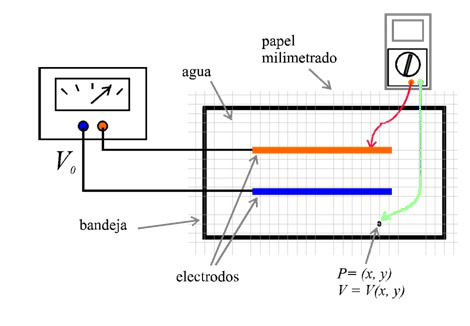
\includegraphics[width=8.5cm]{LG01--000.png}
\caption{Esquema del dispositivo experimental propuesto (bandeja en vista
superior). La bandeja de material aislante contiene agua. Las l\'\i neas
gruesas cont\'\i nuas representan los electrodos met\'alicos. En el punto
de coordenadas $(x,y)$, se mide el valor del potencial el\'ectrico $V(x,y)$.}
    \label{fig:1}
\end{figure}

Habiendo montado el dispositivo experimental, realice unos primeros intentos
exploratorios para determinar el potencial electrost\'atico en diversos puntos
del espacio, asegur\'andose de que comprende c\'omo funciona el sistema. 

Una vez que se haya familiarizado con su funcionamiento y operaci\'on, realice
las siguientes actividades:
\begin{enumerate}
    \item Determine las l\'\i neas equipotenciales en la zona entre los electrodos.
    \item Para la misma configuraci\'on anterior, coloque un conductor entre los 
        electrodos y determine las l\'\i neas equipotenciales de este nuevo 
        arreglo (ver Figura~\ref{fig:2}). En particular, estudie la forma de las  l\'\i neas 
        equipotenciales alrededor del conductor. ?`C\'omo deber\'\i an ser las 
        l\'\i neas equipotenciales dentro del mismo?  
    \item Repita las mediciones reemplazando ahora el conductor por un aislante de forma
        geom\'etrica simple.
\end{enumerate}


\begin{figure}[t!]
    \centering
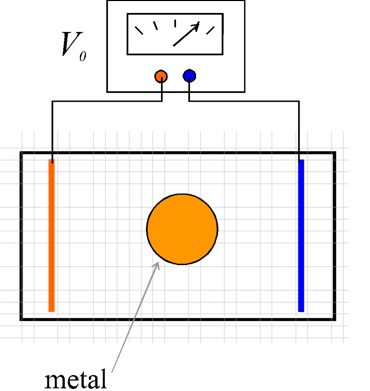
\includegraphics[width=5cm]{LG01--001.png}
\caption{Esquema del segundo dispositivo experimental propuesto (bandeja en vista
superior). La bandeja de material aislante contiene agua. Las l\'\i neas
gruesas cont\'\i nuas representan los electrodos met\'alicos, entre los cuales
se ha dispuesto ahora un medio conductor de forma geom\'etrica simple. Del mismo
modo que antes, en un punto
de coordenadas $(x,y)$, se mide el valor del potencial el\'ectrico $V(x,y)$
para esta nueva configuraci\'on.}
    \label{fig:2}
\end{figure}

\section{C\'omo trabajar en esta gu\'\i a}

\begin{itemize}
    \item Mida por lo menos 6 a 8 puntos para cada equipotencial, con
        separaciones de aproximadamente 1 cm. Luego, en papel milimetrado,
        marque estos puntos y \'unalos con l\'\i neas cont\'\i nuas. Estas son
        las l\'\i neas equipotenciales correspondientes a la geometr\'\i a de
        electrodos (o electrodos y conductor o aislante) elegida. Para cada
        configuraci\'on, determine al menos 10 l\'\i neas equipotenciales,
        tratando de que alguna de ellas se encuentren cerca de cada electrodo y
        algunas en las zonas centrales del arreglo.

    \item Determine las l\'\i neas equipotenciales y las l\'\i neas de campo
        el\'ectrico para por lo menos dos configuraciones de electrodos. En
        cada caso discuta las zonas donde el campo es mayor.

    \item Para el caso del conductor entre los electrodos, observe la
        configuraci\'on de l\'\i neas equipotenciales alrededor del conductor.
        ?`C\'omo son las l\'\i neas de campo sobre la superficie del conductor?

    \item Preste particular atenci\'on a la configuraci\'on en la que se
        dispone un aislante entre los electrodos. En particular estudie las
        l\'\i neas equipotenciales alrededor del aislante. ?`C\'omo son las
        l\'\i neas de campo y el campo mismo sobre su superficie? ?`C\'omo
        puede explicar lo que observa en este caso?
\end{itemize}


\nocite{Alonso1998,Purcell1988,Reitz1996,Trelles1984}
\bibliographystyle{unsrt} 
\bibliography{Bibliografia}

\end{document}
